\section{Exactness}
\label{sec:exactness}

Floating-point addition is not associative, so two correct implementations of the same
formula usually differ in the last bits, and after rounding to 8 bits a few pixels differ by
one grey level. The WSQ specification tolerates that (at least 99.9\% of the pixels equal and
none off by more than one), but a viewer that shows exactly what the reference decoder shows
removes any doubt, and an encoder that writes the reference's bytes can be checked with a
hash. Exactness had to coexist with vectorization; this section shows how.

\subsection{Recording the operation order}

The inverse transform of NBIS walks a pointer back and forth over each line, reflecting at the
ends, and accumulates products in a particular order. Rather than re-deriving that order, the
codec contains a literal port of the two NBIS routines (\code{get\_lets} and \code{join\_lets})
that, instead of computing, \emph{records} for every output sample the list of
(input index, coefficient) pairs in the order NBIS adds them, including the cases where NBIS
overwrites a partial sum. The result is a \emph{schedule} per line length and parity. Evaluating
a schedule in float32, multiply then add, never fused, reproduces NBIS bit for bit; the schedules
are computed once per image size and cached.

Exactness then constrains the order of operations \emph{within} one output, not across outputs.
A vector can therefore hold several lines at once: in the column pass, eight adjacent columns
for AVX2 (Figure~\ref{fig:lanes}); every lane performs exactly the scalar sequence of its line.
For the row pass, the codec detects, from the schedule itself, the long interior run in which
consecutive even outputs (and consecutive odd ones) use the same terms shifted by one sample.
There a vector holds consecutive outputs of the same row, and an interleave merges even and odd
results (Figure~\ref{fig:rowdirect}). The few outputs near the ends of a row, whose terms differ,
are evaluated one at a time from the schedule.

\begin{figure}[ht]
  \centering
  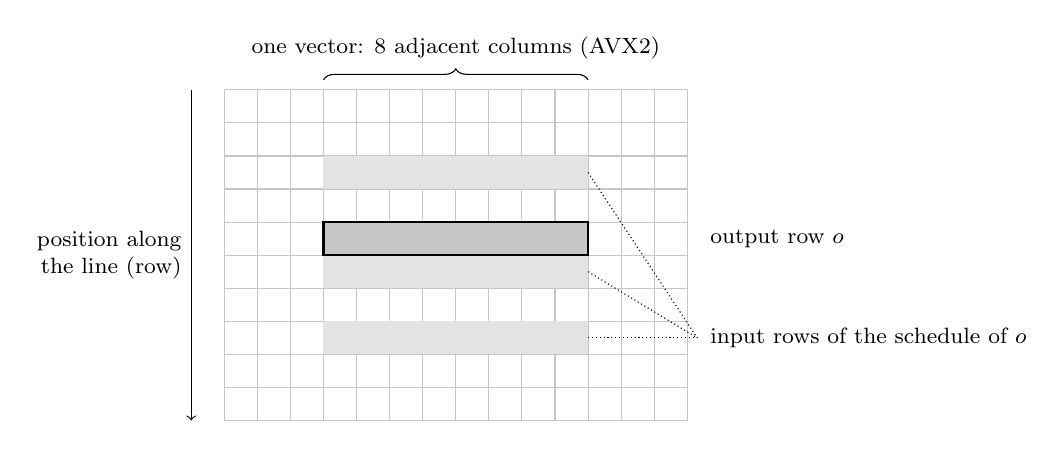
\begin{tikzpicture}[x=0.42cm,y=-0.42cm,font=\footnotesize]
  % a region: columns are lines of the column pass
  \foreach \c in {0,...,13} \foreach \r in {0,...,9} \draw[gray!45] (\c,\r) rectangle (\c+1,\r+1);
  \fill[gray!22] (3,2) rectangle (11,3);
  \fill[gray!22] (3,5) rectangle (11,6);
  \fill[gray!22] (3,7) rectangle (11,8);
  \fill[gray!45] (3,4) rectangle (11,5);
  \draw[line width=0.9pt] (3,4) rectangle (11,5);
  \draw[decorate,decoration={brace,amplitude=4pt}] (3,-0.3) -- (11,-0.3) node[midway,above=4pt] {one vector: 8 adjacent columns (AVX2)};
  \draw[->] (-1,0) -- (-1,10) node[midway,left,align=right] {position along\\the line (row)};
  \node[anchor=west] at (14.4,4.5) {output row $o$};
  \node[anchor=west] at (14.4,7.5) {input rows of the schedule of $o$};
  \draw[densely dotted] (11,2.5) -- (14.3,7.5);
  \draw[densely dotted] (11,5.5) -- (14.3,7.5);
  \draw[densely dotted] (11,7.5) -- (14.3,7.5);
\end{tikzpicture}

  \caption{Column pass: one vector covers adjacent columns, each lane runs the schedule of its
  column, so the operation order of every output is the scalar one.}
  \label{fig:lanes}
\end{figure}

\begin{figure}[ht]
  \centering
  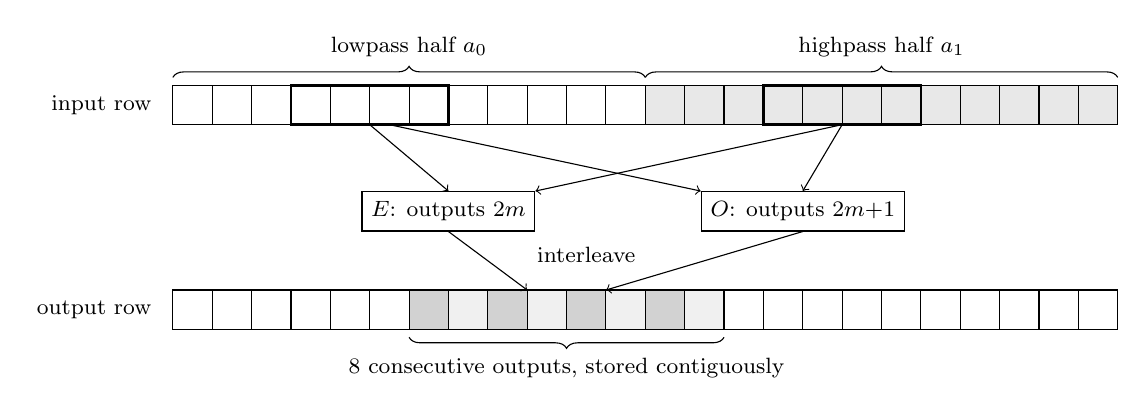
\begin{tikzpicture}[x=0.5cm,y=-0.5cm,font=\footnotesize]
  % input row: lowpass half then highpass half
  \foreach \i in {0,...,11} \draw (\i,0) rectangle (\i+1,1);
  \foreach \i in {12,...,23} \draw[fill=gray!18] (\i,0) rectangle (\i+1,1);
  \node[anchor=east] at (-0.3,0.5) {input row};
  \draw[decorate,decoration={brace,amplitude=4pt}] (0,-0.2) -- (12,-0.2) node[midway,above=4pt] {lowpass half $a_0$};
  \draw[decorate,decoration={brace,amplitude=4pt}] (12,-0.2) -- (24,-0.2) node[midway,above=4pt] {highpass half $a_1$};
  % a vector of 4 consecutive m in each half
  \draw[line width=1pt] (3,0) rectangle (7,1);
  \draw[line width=1pt] (15,0) rectangle (19,1);
  % even and odd vectors
  \node[draw,minimum width=2cm,minimum height=5mm] (E) at (7,3.2) {$E$: outputs $2m$};
  \node[draw,minimum width=2cm,minimum height=5mm] (O) at (16,3.2) {$O$: outputs $2m{+}1$};
  \draw[->] (5,1) -- (E.north);
  \draw[->] (17,1) -- (E.north east);
  \draw[->] (5.5,1) -- (O.north west);
  \draw[->] (17,1) -- (O.north);
  % interleaved output
  \foreach \i in {0,...,23} \draw (\i,5.2) rectangle (\i+1,6.2);
  \foreach \i in {6,8,...,12} \fill[gray!35] (\i,5.2) rectangle (\i+1,6.2);
  \foreach \i in {7,9,...,13} \fill[gray!12] (\i,5.2) rectangle (\i+1,6.2);
  \foreach \i in {6,...,13} \draw (\i,5.2) rectangle (\i+1,6.2);
  \node[anchor=east] at (-0.3,5.7) {output row};
  \draw[->] (E.south) -- (9,5.2);
  \draw[->] (O.south) -- (11,5.2);
  \node at (10.5,4.3) {interleave};
  \draw[decorate,decoration={brace,amplitude=4pt,mirror}] (6,6.4) -- (14,6.4) node[midway,below=4pt] {8 consecutive outputs, stored contiguously};
\end{tikzpicture}

  \caption{Row-direct synthesis: in the interior of a row, the even outputs $2m$ for four
  consecutive $m$ use the same terms shifted by one sample, and so do the odd ones; two vectors
  are computed and interleaved into eight consecutive outputs.}
  \label{fig:rowdirect}
\end{figure}

\subsection{Mixed float and double arithmetic}

NBIS mixes float and double in ways C's promotion rules make easy to miss. The codec mirrors
each case, and two of them could be vectorized in float only after a short proof.
\begin{itemize}
  \item \emph{Scaled integers}: NBIS converts the integer to float and divides by 10 once per
    exponent step, rounding to float after each division; the codec does the same.
  \item \emph{Dequantization}: NBIS adds $Z/2$ in double to a float product and rounds the sum to
    float. The double sum of two floats is exact when their exponents differ by fewer than 29,
    and then rounding it to float gives the correctly rounded float sum, which is what a float
    addition returns. Here the two terms differ by at most a factor of about $|p| \le 65535$, so
    a float addition gives NBIS's result.
  \item \emph{Quantization}: NBIS computes $(\text{short})(t + 1.0)$ in double for a quotient
    $t > 0$, and $(\text{short})(t - 1.0)$ for $t < 0$. Truncation commutes with adding one when the
    sign does not change, so $\mathrm{trunc}(t) \pm 1$ in float gives the same index, with one
    division per coefficient instead of two branches.
  \item \emph{Output}: NBIS adds $0.5$ in double before truncating; for the same reason as above,
    adding $0.5$ in float gives the same pixel.
\end{itemize}
The variance sums and the bit-allocation constant of the encoder keep NBIS's sequential float
accumulation and its double-precision \code{pow} and \code{log} calls, which on Linux resolve to
the same C library NBIS uses.

\subsection{Verification}

Table~\ref{tab:verification} lists what the test suite checks against NBIS. The expected outputs
are 64-bit hashes of what NBIS produced, stored in the repository, so the tests need the public
NIST data but not NBIS itself.

\begin{table}[ht]
  \centering\small
  \begin{tabular}{@{}p{7.4cm}p{6.4cm}@{}}
    \toprule
    check & result \\
    \midrule
    exact decoder, 86 NIST decoder files (9/7, 6/10, 10/10 and 9/11 filter banks), every
    backend (AVX-512 on the server of Section~\ref{sec:server}), 1 and 4 threads & identical pixels in every case \\
    exact encoder, 40 images at 0.75 and 2.25 bits per pixel, every backend & identical bytes in all 80 cases \\
    quantizer indices of the two NIST reference files & identical in all 60 subbands \\
    WebAssembly build (scalar and SIMD), three images & identical pixels \\
    fast decoder against NBIS, 86 files & Annex AA.3 met in every case (at least 99.994\% equal, never more than 1 apart) \\
    fast encoder against NBIS, 80 cases & Annex AA.2 met in every case (size within 0.04\%, bins within 0.015\%) \\
    \bottomrule
  \end{tabular}
  \caption{Exactness checks of the test suite (\code{cargo test} with \code{WSQ\_NIST\_DIR} set).}
  \label{tab:verification}
\end{table}
